\documentclass[border=1pt]{standalone}
\usepackage{fontspec}
\usepackage[dvipsnames,svgnames]{xcolor} % Extended color support
\usepackage{tikz}
\usepackage{pgfplots}
\usepackage{amsmath}
\usepackage{amssymb}
\usepackage{mathtools}
\usepackage{unicode-math}
\usepackage{graphicx}
\usepackage{microtype}
\usepackage{enumitem}

\pgfplotsset{
  compat=1.18
}

%\setmainfont{Libertinus Sans}
%\setsansfont{Libertinus Sans}
%\setmonofont{Libertinus Mono}
%\setmathfont{Libertinus Math}

\setmainfont{Noto Sans}
\setsansfont{Noto Sans}
\setmonofont{Noto Sans Mono}
\setmathfont[
  Path=fonts/,
  Extension=.ttf
]{NotoSansMath-Regular}

\usetikzlibrary{
  calc,
  positioning,
  intersections,
  through,
  angles,
  quotes,
  arrows.meta,
  patterns,
  decorations.pathreplacing,
  decorations.markings,
  decorations.text,
  shapes,
  shapes.geometric,
  matrix,
  fit,
  backgrounds,
  fadings
}

\begin{document}
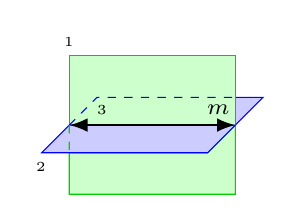
\begin{tikzpicture}[>=Latex]
  \tikzset{
    dimline/.style={
      arrows={Bar[length=0pt,width=14pt]}-{Bar[length=0pt,width=14pt]}
    },
    dot ends/.style={
      {Circle[length=2pt]}-{Circle[length=2pt]}
    },
    %    every path/.style={thick},
    % every node/.style={font=\large}
  }
\coordinate (q4) at (0,0);
\coordinate (q1) at ($(q4)+(0,50pt)$);
\coordinate (q2) at ($(q1)+(60pt,0)$);
\coordinate (q3) at ($(q2)+(0,-50pt)$);

%\draw[red] (q4)--(q1)--(q2)--(q3)--cycle;

\coordinate (p1) at (-10pt,15pt);
\coordinate (p2) at ($(p1)+(20pt,20pt)$);
\coordinate (p3) at ($(p2)+(60pt,0)$);
\coordinate (p4) at ($(p3)+(-20pt,-20pt)$);

%\draw[blue] (p1)--(p2)--(p3)--(p4)--cycle;

\path[name path=p1p2] (p1)--(p2);
\path[name path=p2p3] (p2)--(p3);
\path[name path=p3p4] (p3)--(p4);
\path[name path=p1p4] (p1)--(p4);

\path[name path=q1q4] (q1)--(q4);
\path[name path=q2q3] (q2)--(q3);

\path[name intersections={of=p1p2 and q1q4, by=k1}];
\path[name intersections={of=p3p4 and q2q3, by=k2}];
\path[name intersections={of=p1p4 and q1q4, by=k3}];
\path[name intersections={of=p2p3 and q2q3, by=k4}];

\draw[fill=blue!20,draw=blue] (k2)--(k4)--(p3)--cycle;
\draw[fill=green!20,draw=green!80!black] (k3)--(p4)--(k2)--(q3)--(q4)--cycle;
\draw[fill=green!20,draw=green!80!black] (k1)--(q1)--(q2)--(k2)--cycle;
\draw[fill=blue!20,draw=blue] (p1)--(k1)--(k2)--(p4)--cycle;

\draw[draw=blue,dashed] (k1)--(p2)--(k4);
\draw[draw=green!80!black, dashed] (k1)--(k3);

\draw[thick, <->] (k1)--(k2) node[above,pos=0.9] {\footnotesize $m$}
node[above, pos=0.2] {\tiny $3$};

\node[above] at (q1) {\tiny $1$};
\node[below] at (p1) {\tiny $2$};

\end{tikzpicture}

\end{document}
